\documentclass[9pt,aspectratio=169,xcolor=table]{beamer}

%~~~~~~~~~~~~~~~~~~~~~~~~~~~~~~~~~~~~~~~~~~~~~~~~~~~~~~~~~~~~~~~~~~~~~~~~~~~~~~
% Use roboto Font (recommended)
\usepackage[sfdefault]{roboto}
\usepackage[utf8]{inputenc}
\usepackage[T1]{fontenc}
%~~~~~~~~~~~~~~~~~~~~~~~~~~~~~~~~~~~~~~~~~~~~~~~~~~~~~~~~~~~~~~~~~~~~~~~~~~~~~~

%~~~~~~~~~~~~~~~~~~~~~~~~~~~~~~~~~~~~~~~~~~~~~~~~~~~~~~~~~~~~~~~~~~~~~~~~~~~~~~
% Define where theme files are located. ('/styles')
\usepackage{styles/fluxmacros}
\usefolder{styles}
% Use Flux theme v0.1 beta
% Available style: asphalt, blue, red, green, gray
\usetheme[style=hunter]{flux}
%~~~~~~~~~~~~~~~~~~~~~~~~~~~~~~~~~~~~~~~~~~~~~~~~~~~~~~~~~~~~~~~~~~~~~~~~~~~~~~

%~~~~~~~~~~~~~~~~~~~~~~~~~~~~~~~~~~~~~~~~~~~~~~~~~~~~~~~~~~~~~~~~~~~~~~~~~~~~~~
% Extra packages
\usepackage{booktabs}
\usepackage{colortbl}
\usepackage{ragged2e}
\usepackage{amssymb}
\usepackage{multirow}
\usepackage{tikz}
\usetikzlibrary{arrows.meta, positioning, fit, backgrounds, calc, decorations.pathreplacing}
\setbeamertemplate{itemize items}[square]
\usepackage[scaled=.8]{beramono}
\usepackage{listings}
\usepackage{styles/lstlangarm}
\usepackage{array}
\definecolor{bgcolor}{HTML}{F2E9E9}
% lstlangarm.sty references \color{mauve} for string literals but never defines
% it -- only fires when a listing contains a string. Define it here.
\definecolor{mauve}{rgb}{0.58,0,0.82}
% lstlangarm's C style sets commentstyle=green!20, which is unreadable on the
% pink listing background. Darken it globally.
\lstset{commentstyle=\color{green!45!black}}
% ragged-right fixed-width column -- must be defined in the preamble, never
% inside a frame (\newcolumntype's #1 breaks beamer's frame scanner)
\newcolumntype{R}[1]{>{\RaggedRight\arraybackslash}p{#1}}
%~~~~~~~~~~~~~~~~~~~~~~~~~~~~~~~~~~~~~~~~~~~~~~~~~~~~~~~~~~~~~~~~~~~~~~~~~~~~~~
% Table striping: odd rows white, even rows very light gray.
% Needs \documentclass[...,xcolor=table]{beamer} (beamer loads xcolor itself,
% so the option must go on the class, not \usepackage).
\definecolor{stripe}{gray}{0.94}
% \striped makes body rows alternate white, gray, white, ... starting white.
% \rowcolors counts from the first coloured body row; the header is not counted.
\newcommand{\striped}{\rowcolors{1}{white}{stripe}}
%~~~~~~~~~~~~~~~~~~~~~~~~~~~~~~~~~~~~~~~~~~~~~~~~~~~~~~~~~~~~~~~~~~~~~~~~~~~~~~

%~~~~~~~~~~~~~~~~~~~~~~~~~~~~~~~~~~~~~~~~~~~~~~~~~~~~~~~~~~~~~~~~~~~~~~~~~~~~~~
% TikZ block styles -- matches ch1/ch2
% Colour variables are named identically in the book's stm32primer.tex, so any
% tikzpicture using only the \tikzset{...} styles below can be copied verbatim
% between slides and book. Only the \definecolor/\colorlet VALUES differ: the
% book is printed, so it keeps every stroke pure black with muted fills. These
% slides are projected, so both fill AND stroke are bright and saturated to
% grab attention -- see stm32primer.tex for the print palette.
\definecolor{blkfill}{HTML}{DDEEDD}
\definecolor{blkline}{HTML}{355E3B}
\definecolor{accentfill}{HTML}{FFE0B2}
\definecolor{accentline}{HTML}{E65100}
\definecolor{memfill}{HTML}{DFF5DA}
\definecolor{memline}{HTML}{2E7D32}
\definecolor{cellfill}{HTML}{FFFFFF}
\definecolor{cellline}{HTML}{424242}
\definecolor{bitmaskfill}{HTML}{DCEBFF}
\definecolor{bitmaskline}{HTML}{1565C0}
\definecolor{bithitfill}{HTML}{FFE0B2}
\definecolor{bithitline}{HTML}{E65100}
\tikzset{
  blk/.style   = {rectangle, rounded corners=2pt, draw=blkline, fill=blkfill,
                  thick, align=center, font=\small, minimum height=9mm, inner sep=3pt},
  cpublk/.style= {rectangle, rounded corners=2pt, draw=accentline, fill=accentfill,
                  thick, align=center, font=\small\bfseries, minimum height=9mm, inner sep=3pt},
  memblk/.style= {rectangle, rounded corners=2pt, draw=memline, fill=memfill,
                  thick, align=center, font=\small, minimum height=9mm, inner sep=3pt},
  cell/.style  = {rectangle, draw=cellline, fill=cellfill, align=center,
                  font=\small\ttfamily, minimum height=7mm, inner sep=2pt},
  bitcell/.style={rectangle, draw=cellline, fill=cellfill, thick,
                  minimum width=5.4mm, minimum height=5.4mm, inner sep=0pt,
                  font=\scriptsize\ttfamily, anchor=center},
  bitmask/.style={bitcell, fill=bitmaskfill, draw=bitmaskline},
  bithit/.style ={bitcell, fill=bithitfill, draw=bithitline, font=\scriptsize\ttfamily\bfseries},
  rowlab/.style ={font=\scriptsize, text=Gray, anchor=east},
  oplab/.style  ={font=\scriptsize\itshape, text=Gray, anchor=west},
  lbl/.style   = {font=\scriptsize, text=Gray},
  flow/.style  = {-{Stealth[length=2mm]}, thick, draw=blkline},
  busline/.style={thick, draw=cellline},
}
% NOTE (theme quirks -- all fail SILENTLY, always page through the PDF):
%  - a second \\ inside a nested {...} group in a TikZ node breaks parsing
%  - {\small ...} wrapped around a nested itemize eats the frame title + list
%  - \usebeamercolor on a [plain] frame falls through to an unstyled default
%  - \newcolumntype inside a frame breaks beamer's frame scanner
%  - lstlisting needs \begin{frame}[fragile]
%  - a TikZ picture wider than its column silently overflows into neighbours
%~~~~~~~~~~~~~~~~~~~~~~~~~~~~~~~~~~~~~~~~~~~~~~~~~~~~~~~~~~~~~~~~~~~~~~~~~~~~~~

%%%%%%%%%%%%%%%%%%%%%%%%%%%%%%%%%%%
%% BEGIN CONDITIONAL COMPILATION %%
%%%%%%%%%%%%%%%%%%%%%%%%%%%%%%%%%%%
\newif\ifwebex
%\webextrue % uncomment to generate section separator
\ifwebex
\AtBeginSection[]{
  \begin{frame}
  \vfill
  \centering
  \begin{beamercolorbox}[sep=8pt,center,shadow=true,rounded=true]{title}
    \usebeamerfont{title}\insertsectionhead\par%
  \end{beamercolorbox}
  \vfill
  \end{frame}
}
\else
\AtBeginSection[]
{
{
    \setbeamercolor{background canvas}{bg=yellow!10}
    \begin{frame}[plain]
        \frametitle{Table of Contents}
        \tableofcontents[currentsection]
    \end{frame}
}
}
\fi
%%%%%%%%%%%%%%%%%%%%%%%%%%%%%%%%%%%
%% END CONDITIONAL COMPILATION   %%
%%%%%%%%%%%%%%%%%%%%%%%%%%%%%%%%%%%

%~~~~~~~~~~~~~~~~~~~~~~~~~~~~~~~~~~~~~~~~~~~~~~~~~~~~~~~~~~~~~~~~~~~~~~~~~~~~~~
% Information
\title{Combinational Logic Design}
\subtitle{\emph{Contemporary Digital Electronic Systems} --- Chapter 7}
\author{Mun\'{i}m Zabidi}
\institute{\color{primary}Faculty of Electrical Engineering, Universiti Teknologi Malaysia}
\date{\today}
\titlegraphic{assets/logoutmwhite.png}
\graphicspath{{.}{../fig/}}
%~~~~~~~~~~~~~~~~~~~~~~~~~~~~~~~~~~~~~~~~~~~~~~~~~~~~~~~~~~~~~~~~~~~~~~~~~~~~~~

\begin{document}

\titlepage

%===============================================================================
\section{Why This Chapter}
%===============================================================================

\begin{frame}{Why This Chapter Matters}
  \begin{columns}[c]
  \begin{column}{.47\textwidth}
    The earlier chapters each built one skill. This chapter combines them into a complete, repeatable \alert{design procedure}: understand the problem, specify a truth table, minimise, draw the schematic, and verify. Every later design chapter follows this template.
  \end{column}
  \begin{column}{.51\textwidth}
    \begin{block}{After this chapter, you can:}
    {\small
    \begin{enumerate}\itemsep2pt
      \item Translate an English specification into a truth table.
      \item Apply the combinational-design procedure.
      \item Design a two-level NAND-only or NOR-only implementation.
      \item Verify a circuit against its specification by simulation.
    \end{enumerate}}
    \end{block}
  \end{column}
  \end{columns}
\end{frame}

\begin{frame}{An Opening Question}
  \leavevmode\vspace{4mm}
  \begin{center}
  \fbox{\parbox{.78\textwidth}{\centering\vspace{2mm}
  \large If a combinational circuit's output depends only on its \alert{current} inputs, what is it allowed to \alert{remember}?
  \vspace{2mm}}}
  \end{center}
  \vspace{4mm}
  Answer: nothing. Change an input, wait $t_{pd}$, and the output follows. There is no past, no state and no clock.
\end{frame}

%===============================================================================
\section{Design Procedure}
%===============================================================================

\begin{frame}{The Design Procedure}
  \centering
  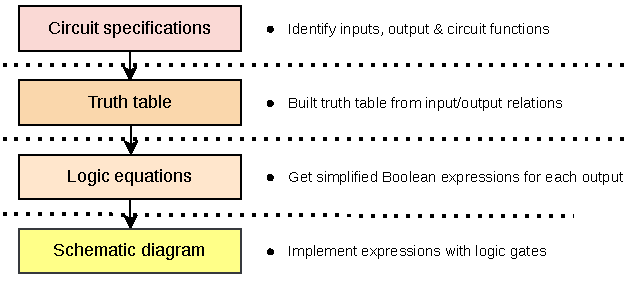
\includegraphics[width=.75\textwidth]{combinational_synthesis}
  \begin{enumerate}\small\itemsep2pt
    \item \alert{Specify}: identify the inputs and outputs and the relationship between them.
    \item \alert{Truth table}: describe that relationship for every input combination.
    \item \alert{Minimise}: derive a simplified SOP for each output (K-map or Boolean algebra).
    \item \alert{Implement} with gates and \alert{verify} in simulation.
  \end{enumerate}
\end{frame}

\begin{frame}{Example 1: Majority Decider}
  \begin{columns}[c]
  \begin{column}{.5\textwidth}
    \centering
    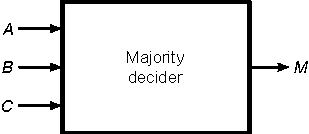
\includegraphics[width=.8\textwidth]{majority_tl}\\[2mm]
    \small \alert{Step 1.} Three inputs $A, B, C$; one output $M$ that is 1 when two or three inputs are 1.
  \end{column}
  \begin{column}{.25\textwidth}
    \centering\small
    \begin{tabular}{ccc|c}
      \toprule
      $A$ & $B$ & $C$ & $M$ \\
      \midrule
      0 & 0 & 0 & 0 \\ 0 & 0 & 1 & 0 \\ 0 & 1 & 0 & 0 \\ 0 & 1 & 1 & 1 \\
      1 & 0 & 0 & 0 \\ 1 & 0 & 1 & 1 \\ 1 & 1 & 0 & 1 \\ 1 & 1 & 1 & 1 \\
      \bottomrule
    \end{tabular}
  \end{column}
  \begin{column}{.22\textwidth}
    \small \alert{Step 2.} $M = 1$ for $m_3, m_5, m_6, m_7$.
  \end{column}
  \end{columns}
\end{frame}

\begin{frame}{Majority Decider: Equation and Schematic}
  \begin{columns}[c]
  \begin{column}{.4\textwidth}
    \centering
    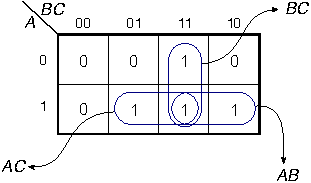
\includegraphics[width=.9\textwidth]{majority_km}\\[2mm]
    {\small \alert{Step 3.} Three overlapping pair loops; $ABC$ is used in all three.}
    \begin{block}{}
      $M = AB + AC + BC$
    \end{block}
  \end{column}
  \begin{column}{.58\textwidth}
    \centering
    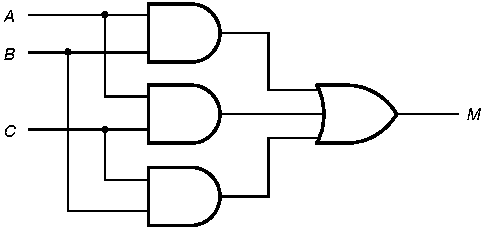
\includegraphics[width=\textwidth]{majority_sc}\\[2mm]
    {\small \alert{Step 4.} Each product term is a 2-input AND; a 3-input OR combines them.}
  \end{column}
  \end{columns}
\end{frame}

\begin{frame}{Example 2: BCD to Excess-3 Converter}
  \begin{columns}[c]
  \begin{column}{.4\textwidth}
    \centering
    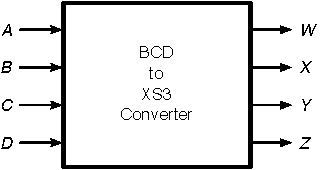
\includegraphics[width=.9\textwidth]{bcd2xs3_top}
    \begin{itemize}\small\itemsep3pt
      \item 4 inputs $ABCD$ (BCD), 4 outputs $WXYZ$ (XS-3).
      \item Inputs 1010 to 1111 never occur: all outputs are \alert{don't cares}.
    \end{itemize}
  \end{column}
  \begin{column}{.58\textwidth}
    \centering\tiny\striped
    \begin{tabular}{cccc|cccc}
      \toprule
      $A$ & $B$ & $C$ & $D$ & $W$ & $X$ & $Y$ & $Z$ \\
      \midrule
      0&0&0&0&0&0&1&1 \\ 0&0&0&1&0&1&0&0 \\ 0&0&1&0&0&1&0&1 \\ 0&0&1&1&0&1&1&0 \\
      0&1&0&0&0&1&1&1 \\ 0&1&0&1&1&0&0&0 \\ 0&1&1&0&1&0&0&1 \\ 0&1&1&1&1&0&1&0 \\
      1&0&0&0&1&0&1&1 \\ 1&0&0&1&1&1&0&0 \\
      1&0&1&0&$\times$&$\times$&$\times$&$\times$ \\ 1&0&1&1&$\times$&$\times$&$\times$&$\times$ \\
      1&1&0&0&$\times$&$\times$&$\times$&$\times$ \\ 1&1&0&1&$\times$&$\times$&$\times$&$\times$ \\
      1&1&1&0&$\times$&$\times$&$\times$&$\times$ \\ 1&1&1&1&$\times$&$\times$&$\times$&$\times$ \\
      \bottomrule
    \end{tabular}
  \end{column}
  \end{columns}
\end{frame}

\begin{frame}{BCD to XS-3: Four K-Maps}
  \centering
  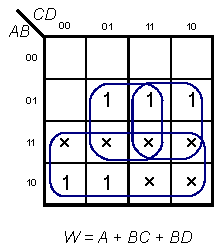
\includegraphics[height=.3\textheight]{bcd2xs3_km1}\hspace{3mm}
  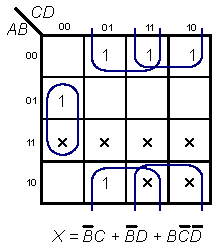
\includegraphics[height=.3\textheight]{bcd2xs3_km2}\hspace{3mm}
  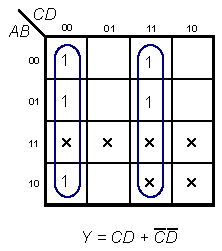
\includegraphics[height=.3\textheight]{bcd2xs3_km3}\hspace{3mm}
  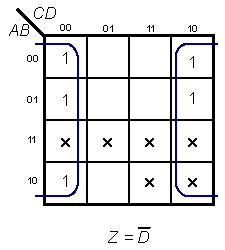
\includegraphics[height=.3\textheight]{bcd2xs3_km4}
  \begin{itemize}\small
    \item One map per output bit. Include don't cares in a loop whenever it makes the loop larger.
  \end{itemize}
  \begin{block}{Simplified equations}
    \small
    $W = A + BC + BD \qquad X = \overline{B}C + \overline{B}D + B\overline{C}\,\overline{D}$\\
    $Y = CD + \overline{C}\,\overline{D} \qquad\qquad Z = \overline{D}$
  \end{block}
\end{frame}

\begin{frame}{BCD to XS-3: Schematic}
  \begin{columns}[c]
  \begin{column}{.45\textwidth}
    \centering
    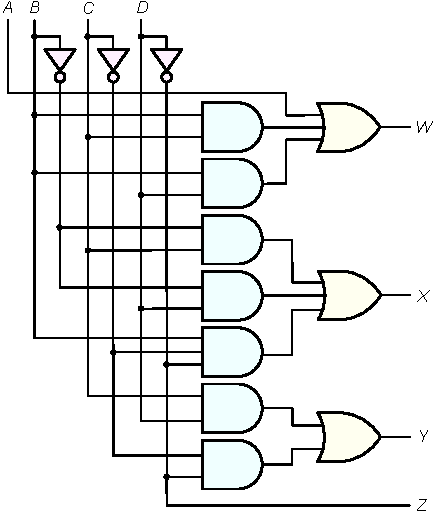
\includegraphics[height=.68\textheight]{bcd2xs3_sc}
  \end{column}
  \begin{column}{.53\textwidth}
    \begin{itemize}\small\itemsep4pt
      \item The same AND--OR translation as the majority circuit: one gate per product term, one OR per output.
      \item Four outputs make the schematic larger, but no new technique is needed.
    \end{itemize}
  \end{column}
  \end{columns}
\end{frame}

%===============================================================================
\section{Universal Gates}
%===============================================================================

\begin{frame}{Why Universal Gates?}
  \begin{itemize}\small\itemsep3pt
    \item Using as few gate types as possible reduces design complexity and cost, so ICs are built from \alert{NAND} or \alert{NOR}.
    \item De Morgan's theorems show why: $AB = \overline{\overline{A}+\overline{B}}$ and $A+B = \overline{\overline{A}\,\overline{B}}$.
    \item A NAND gate equals an OR gate with inverted inputs: $\overline{AB} = \overline{A}+\overline{B}$.
  \end{itemize}
  \centering
  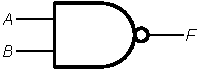
\includegraphics[height=.12\textheight]{universal_nand2}\hspace{10mm}
  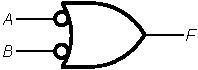
\includegraphics[height=.12\textheight]{universal_bor2}\\[3mm]
  \footnotesize\striped
  \begin{tabular}{cc|cc|cc}
    \toprule
    $A$ & $B$ & $\overline{A}$ & $\overline{B}$ & $\overline{AB}$ & $\overline{A}+\overline{B}$ \\
    \midrule
    0&0&1&1&1&1 \\ 0&1&1&0&1&1 \\ 1&0&0&1&1&1 \\ 1&1&0&0&0&0 \\
    \bottomrule
  \end{tabular}
\end{frame}

\begin{frame}{Building Gates from NAND}
  \begin{columns}[c]
  \begin{column}{.5\textwidth}
    \centering
    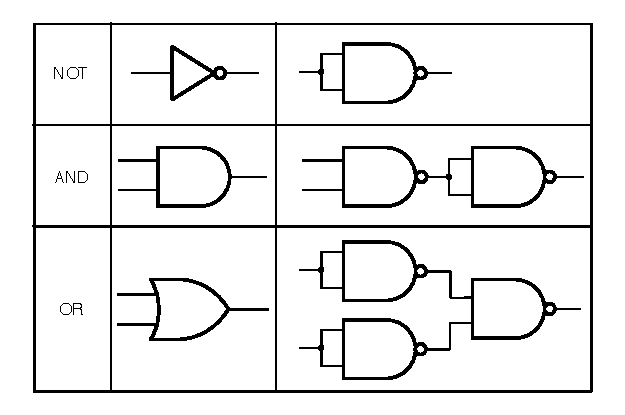
\includegraphics[width=\textwidth]{variasi-nand}
  \end{column}
  \begin{column}{.48\textwidth}
    \begin{block}{NOT from NAND}
      \small Tie the inputs together: $F = \overline{A\cdot A} = \overline{A}$ (idempotent law). Tying NOR inputs works the same way.
    \end{block}
    \begin{itemize}\small\itemsep3pt
      \item With NOT available, NAND gates give AND and OR too.
      \item XOR can also be built from four NAND gates.
    \end{itemize}
    \centering
    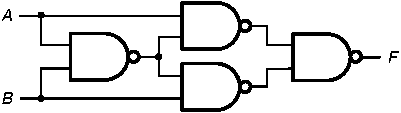
\includegraphics[width=.8\textwidth]{xor_from_nand}
  \end{column}
  \end{columns}
\end{frame}

\begin{frame}{NOR Is Universal Too}
  \begin{columns}[c]
  \begin{column}{.5\textwidth}
    \centering
    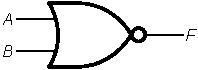
\includegraphics[height=.1\textheight]{universal_nor2}\hspace{6mm}
    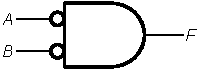
\includegraphics[height=.1\textheight]{universal_band2}\\[2mm]
    \footnotesize\striped
    \begin{tabular}{cc|cc|cc}
      \toprule
      $A$ & $B$ & $\overline{A}$ & $\overline{B}$ & $\overline{A+B}$ & $\overline{A}\,\overline{B}$ \\
      \midrule
      0&0&1&1&1&1 \\ 0&1&1&0&0&0 \\ 1&0&0&1&0&0 \\ 1&1&0&0&0&0 \\
      \bottomrule
    \end{tabular}\\[2mm]
    {\small NOR = AND with inverted inputs.}
  \end{column}
  \begin{column}{.48\textwidth}
    \centering
    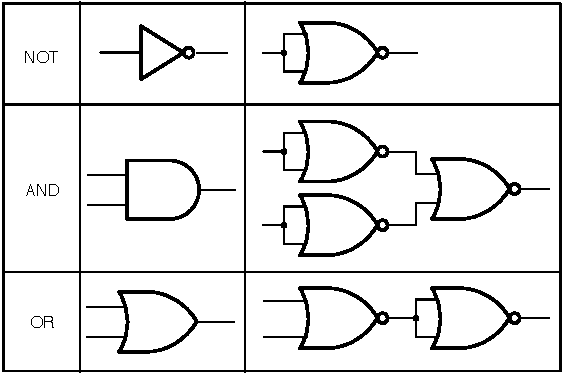
\includegraphics[width=.9\textwidth]{variasi-nor}
  \end{column}
  \end{columns}
\end{frame}

%===============================================================================
\section{NAND-NAND Networks}
%===============================================================================

\begin{frame}{Bubble Pushing}
  \begin{itemize}\small\itemsep3pt
    \item Start from the AND--OR--NOT schematic. Only AND and OR gates are converted; NOT gates stay.
    \item Add \alert{pairs of bubbles}: two consecutive bubbles cancel.
    \item Slide bubbles along a wire until they meet a gate. Gates with bubbles become NAND (or NOR) gates.
  \end{itemize}
  \centering
  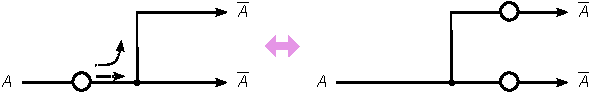
\includegraphics[width=.7\textwidth]{bubblesright}\\[1mm]
  {\scriptsize Pushing bubbles to the right}\\[2mm]
  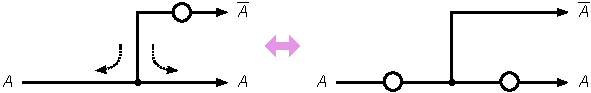
\includegraphics[width=.7\textwidth]{bubblesleft}\\[1mm]
  {\scriptsize Pushing bubbles to the left}
\end{frame}

\begin{frame}{Example: $F = AB + B\overline{C}$}
  \centering
  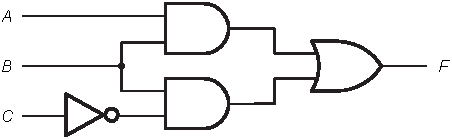
\includegraphics[height=.17\textheight]{nandnand_1a}\hspace{3mm}$\Rightarrow$\hspace{3mm}
  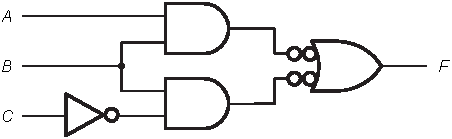
\includegraphics[height=.17\textheight]{nandnand_1b}\hspace{3mm}$\Rightarrow$\hspace{3mm}
  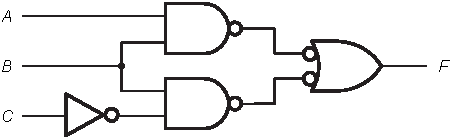
\includegraphics[height=.17\textheight]{nandnand_1c}
  \begin{itemize}\small\itemsep3pt
    \item Add double bubbles between the AND and OR gates.
    \item Slide the left bubble of each pair back to the AND output: the AND gates become NAND.
    \item The OR gate with inverted inputs is also a NAND, by De Morgan. The function is unchanged.
  \end{itemize}
\end{frame}

\begin{frame}{Examples: Extra Inverter, Cancelled Inverter}
  \begin{columns}[t]
  \begin{column}{.5\textwidth}
    \centering\small $F = A\overline{B} + C$\\[1mm]
    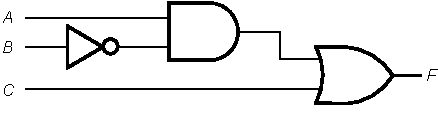
\includegraphics[width=.78\textwidth]{nandnand_2a}\\[1mm]
    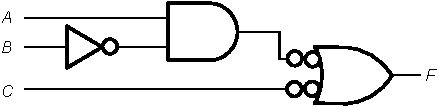
\includegraphics[width=.78\textwidth]{nandnand_2b}\\[1mm]
    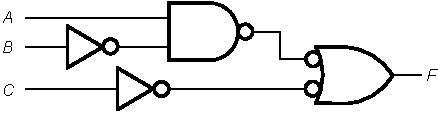
\includegraphics[width=.78\textwidth]{nandnand_2c}\\[1mm]
    {\footnotesize Two bubbles on the OR input need an added inverter.}
  \end{column}
  \begin{column}{.5\textwidth}
    \centering\small $F = A\overline{C} + \overline{B} + BC$\\[1mm]
    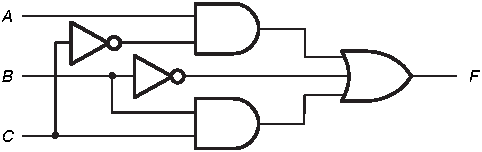
\includegraphics[width=.78\textwidth]{nandnand_3a}\\[1mm]
    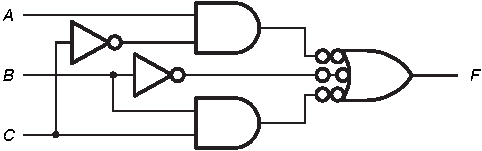
\includegraphics[width=.78\textwidth]{nandnand_3b}\\[1mm]
    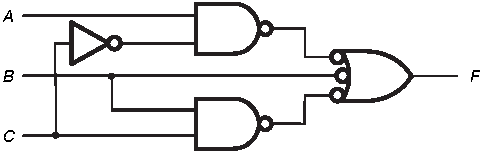
\includegraphics[width=.78\textwidth]{nandnand_3c}\\[1mm]
    {\footnotesize Three bubbles on the middle input: two cancel and the inverter disappears.}
  \end{column}
  \end{columns}
\end{frame}

%===============================================================================
\section{Mixed Logic}
%===============================================================================

\begin{frame}{Positive and Negative Logic}
  \begin{columns}[c]
  \begin{column}{.5\textwidth}
    \begin{itemize}\small\itemsep3pt
      \item \alert{Positive logic}: 1 is the higher voltage. \alert{Negative logic}: 1 is the lower voltage.
      \item The same device is an AND in positive logic and an OR in negative logic.
      \item Mixed logic separates the \emph{functional description} from the \emph{physical implementation}.
    \end{itemize}
    \centering\small\striped
    \begin{tabular}{rcl}
      AND (pos) & $\Leftrightarrow$ & OR (neg) \\
      OR (pos) & $\Leftrightarrow$ & AND (neg) \\
      NAND (pos) & $\Leftrightarrow$ & NOR (neg) \\
      NOR (pos) & $\Leftrightarrow$ & NAND (neg) \\
    \end{tabular}
  \end{column}
  \begin{column}{.48\textwidth}
    \centering
    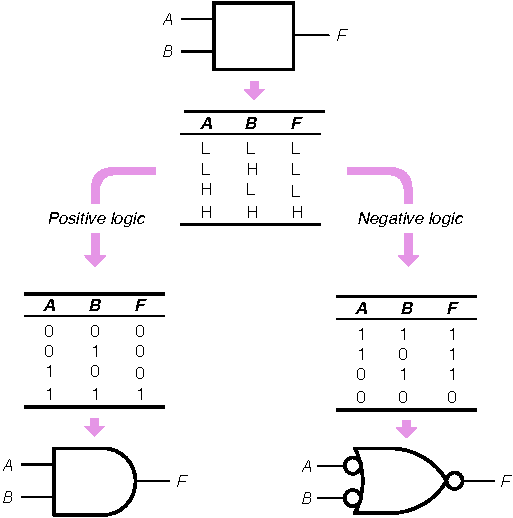
\includegraphics[height=.66\textheight]{posvsneglogic}
  \end{column}
  \end{columns}
\end{frame}

\begin{frame}{De Morgan Equivalent Symbols}
  \begin{columns}[c]
  \begin{column}{.4\textwidth}
    \centering
    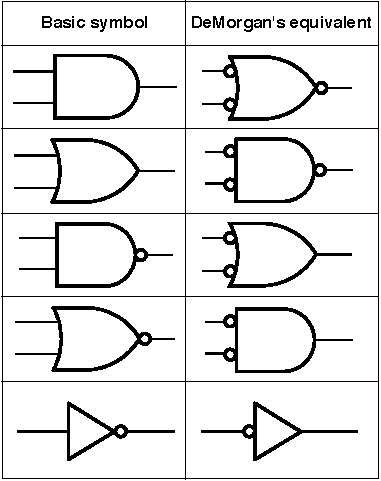
\includegraphics[height=.66\textheight]{demorgan_equivalents}
  \end{column}
  \begin{column}{.58\textwidth}
    \begin{block}{To get the alternative symbol}
      \small
      \begin{enumerate}\itemsep2pt
        \item Invert all inputs and outputs: add a bubble where there is none, remove one where there is.
        \item Switch the symbol: AND to OR, OR to AND. For NOT, move the bubble.
      \end{enumerate}
    \end{block}
    \small Example: NAND (AND with output bubble) becomes OR with bubbles on all inputs.
  \end{column}
  \end{columns}
\end{frame}

\begin{frame}{Choosing the Symbol; Active-Low Signals}
  \begin{columns}[c]
  \begin{column}{.5\textwidth}
    \centering
    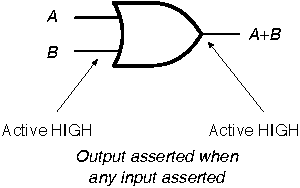
\includegraphics[height=.2\textheight]{poslogic_OR}\hspace{4mm}
    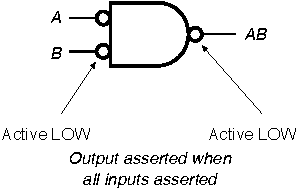
\includegraphics[height=.2\textheight]{neglogic_AND}\\[1mm]
    {\small Positive-logic OR \hspace{.05\textwidth} Negative-logic AND}
    \begin{itemize}\small\itemsep3pt
      \item Describe the function in words first (``output active when all inputs are active'' is AND), then add bubbles for the signal polarity.
    \end{itemize}
  \end{column}
  \begin{column}{.48\textwidth}
    \begin{itemize}\small\itemsep3pt
      \item \alert{Active-low} signals reduce errors in noisy environments and are used for control signals between chips.
      \item Notation: $\overline{RESET}$, \textit{RESETn}, \textit{RESET*}.
      \item Dual-meaning names: \textit{READ}/$\overline{\textit{WRITE}}$, \textit{M}/$\overline{IO}$ (high / low meanings).
    \end{itemize}
  \end{column}
  \end{columns}
\end{frame}

%===============================================================================
\section{NAND Gate ICs}
%===============================================================================

\begin{frame}{NAND Gate ICs}
  \centering
  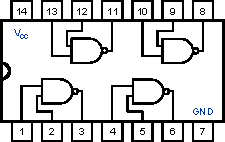
\includegraphics[height=.2\textheight]{inside_7400}\hspace{3mm}
  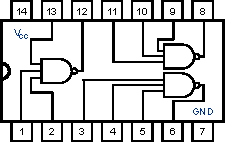
\includegraphics[height=.2\textheight]{inside_7410}\hspace{3mm}
  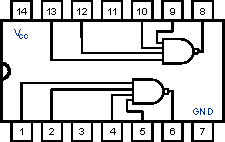
\includegraphics[height=.2\textheight]{inside_7420}\hspace{3mm}
  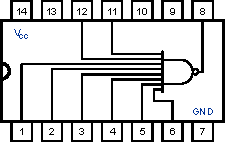
\includegraphics[height=.2\textheight]{inside_7430}\\[1mm]
  {\small 74x00 \hspace{.1\textwidth} 74x10 \hspace{.1\textwidth} 74x20 \hspace{.1\textwidth} 74x30}
  \begin{itemize}\small\itemsep3pt
    \item NAND gates have long been sold in many IC types. These TTL chips are historical but still illustrate the principle.
    \item An equivalent function can be built with different gate mixes and different hardware.
  \end{itemize}
\end{frame}

\begin{frame}{Example: 2:1 Mux in One IC}
  \centering
  {\small $Y = S'A + SB$}\\[1mm]
  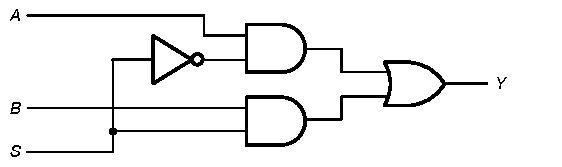
\includegraphics[height=.2\textheight]{orcad2i}\\
  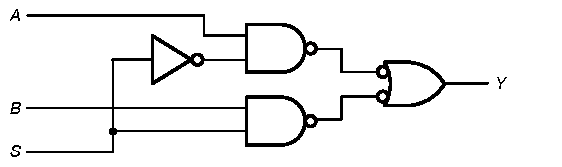
\includegraphics[height=.2\textheight]{orcad2ii}\\
  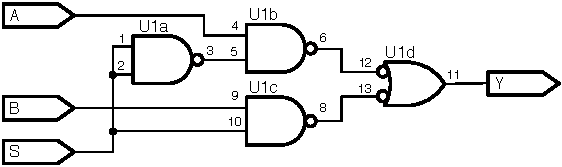
\includegraphics[height=.2\textheight]{orcad2iii}\\[1mm]
  {\footnotesize Original (inverter, 2 AND, 1 OR = 3 ICs) $\to$ all NAND/NOT $\to$ one 74x00 with ports and pins numbered.}
\end{frame}

\begin{frame}{Is It Still Worth Doing?}
  \begin{itemize}\small\itemsep4pt
    \item NAND-based design can cut ICs, wiring, board space and cost. It does not automatically cut power or delay.
    \item Modern systems use microcontrollers, CPLDs, FPGAs or highly integrated logic, not discrete TTL gates.
    \item NAND implementations remain a good \alert{teaching tool}: they show universality.
  \end{itemize}
\end{frame}

%===============================================================================
\section{Summary}
%===============================================================================

\begin{frame}{Summary}
  \begin{itemize}\itemsep3pt\small
    \item Design is: specify $\to$ truth table $\to$ minimise $\to$ draw $\to$ verify.
    \item A combinational circuit has no memory: its output is a pure function of its current inputs.
    \item An AND--OR--NOT schematic converts mechanically to NAND-only (or NOR-only) with De Morgan's laws and bubble pushing.
    \item Verify the final circuit against the specification by simulation.
  \end{itemize}
  \begin{block}{Looking ahead}
    Chapter 8 introduces standard modules (decoders, encoders, multiplexers, demultiplexers) that you compose instead of designing from scratch.
  \end{block}
\end{frame}

\end{document}
